\subsection{Sensors Output Attack}

This attack is carried out adding four extra FMUs between the \code{controller}
and the \code{sensor} FMUs, one for each sensor.

This attack can be performed in two different ways:
\begin{enumerate}
	\item Interval Mode: in this mode the attack is performed once, for an
		interval of time defined by the attacker, starting from an
		instant chosen by the attacker.
	\item Cyclic Mode: the attack is performed periodically.
\end{enumerate}

The attacker can tune the attack by changing the following parameters:
\begin{itemize}
	\item \code{Real attack\_time}: The time at which the attack starts.
	\item \code{Real attack\_duration}: The duration of the attack.
	\item \code{Real attack\_value}: The percentage increment (or decrement,
		if negative) to apply to the output of the sensor \exgratia{A
		value of \(0.5\) makes the output to increment by the
		\(50\%\).}.
	\item \code{Bool cyclic}: if \code{true} the attack is performed
		periodically.
\end{itemize}

The FMU implementation is shown in \lstref{lst:sensorsoutputatk}.

\lstinputlisting[language=C, label={lst:sensorsoutputatk},
caption={Sensors Output Attack FMU}]{sensors-output-attack.c}

In \figref{fig:sensorsoutputatkresult} we can see the result of the attack. In
this case the attack is performed only on the left sensors at time \(5\) and
their output are decreased by the \(50\%\). Thus, the robot will correctly
follow the first curve (black to the left). Then, at time \(10\), the same
attack is also applied to the right sensors, so the robot will start proceeding
forward (black both to the right and to the left). At time \(15\) the attack on
the left sensors ends, so the robot will see black to the right but the correct
value to the left (black or white): this tricks the robot to (mainly) make a
turn to the right. Then, at time \(20\), the attack ends so the next time the
robot will hit against the line it will start to correctly follow it again.

\begin{figure}[htb]
	\centering
	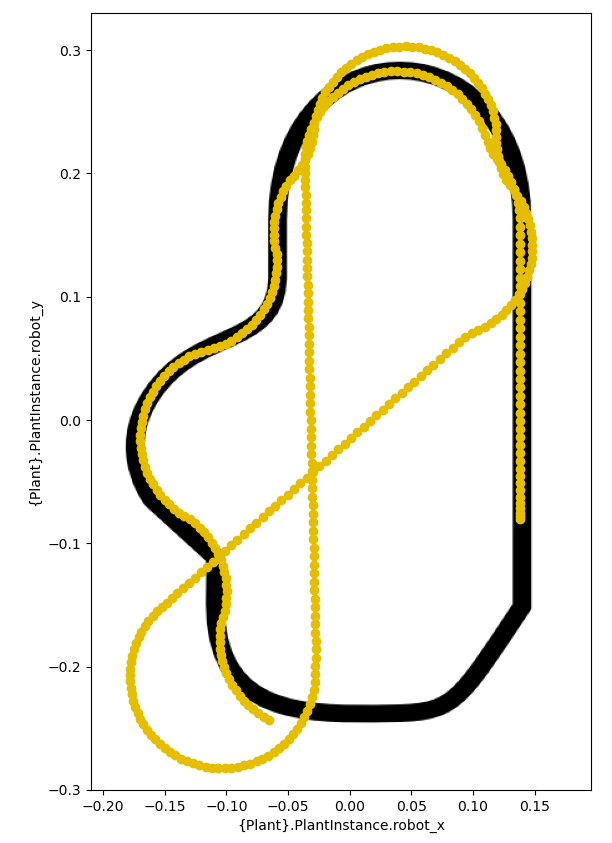
\includegraphics[width=0.5\textwidth]{sensors-output-attack}
	\caption{Line follower robot path when
	attacked}\label{fig:sensorsoutputatkresult}
\end{figure}
